\section{Purpose}
Experiment~1 establishes the reference detector: an Autoencoder trained on normal recordings only and used through its reconstruction error. Everything else in the project builds on the fourteen models trained here, so this chapter also fixes the training protocol and documents how the training was actually run.

\section{Training protocol}\label{sec:protocol}
The problem statement specifies that Model~A uses the 990 source-domain recordings and Model~B the 990 source plus 10 target recordings. We followed this literally: each model is trained on \emph{all} the normal recordings of its configuration, a protocol we call \texttt{spec\_full} in the code. The consequence has to be stated clearly, because it shapes the rest of the report. Since no recording is held out, there is no validation set, no validation loss and no early stopping; the checkpoint after the hundredth epoch is the model. This is also what the official baseline does. The training-loss curve is monitored for convergence (Figure~\ref{fig:losses}) and snapshots are kept every ten epochs, but nothing in the training procedure can detect overfitting. An alternative protocol with a 10\,\% hold-out was implemented in the notebook for an earlier single-machine prototype; it was not used for any of the models reported here.

\section{How the training was run}
All fourteen models were trained on 9~November~2026 in a single Google Colab session with a CUDA GPU runtime. The session log records \texttt{device=cuda} at start, and every checkpoint stores \texttt{device: cuda} together with its start and finish time. The machines were processed one after another from 16:48 to 20:06 UTC, a total of 3\,h\,17\,min including archive extraction, the full audit and feature caching; the per-model training times in Table~\ref{tab:training} add up to 186.5 minutes. A second Colab session on 10~November ran on a CPU runtime and did nothing but re-assemble and verify the handover archive, which is why the environment file written last records \texttt{device: cpu}. No model was trained or modified in that session. The GPU model itself is not recorded in the logs, so we do not name one.

\begin{table}[!htb]
\centering
\caption{Training summary for the 14 models (spec\_full protocol: fixed 100 epochs, final-epoch checkpoint, no validation set). Training executed on a CUDA GPU in Google Colab on 9 November 2026.}
\label{tab:training}
\footnotesize
\renewcommand{\arraystretch}{1.18}
\resizebox{\textwidth}{!}{\begin{tabular}{lrrrrrrr}
\toprule
Machine & Model & Source rec. & Target rec. & Train windows & Epochs & Final train MSE & Minutes \\
\midrule
ToyCar & A & 990 & 0 & 336600 & 100 & 0.474 & 14.600 \\
ToyCar & B & 990 & 10 & 340000 & 100 & 0.475 & 13.000 \\
ToyCarEmu & A & 990 & 0 & 368280 & 100 & 0.496 & 16.300 \\
ToyCarEmu & B & 990 & 10 & 372000 & 100 & 0.496 & 14.400 \\
Fan & A & 990 & 0 & 305910 & 100 & 0.729 & 13.700 \\
Fan & B & 990 & 10 & 309000 & 100 & 0.731 & 11.900 \\
GearboxEmu & A & 990 & 0 & 305910 & 100 & 0.376 & 13.600 \\
GearboxEmu & B & 990 & 10 & 309000 & 100 & 0.377 & 11.900 \\
BearingEmu & A & 990 & 0 & 305910 & 100 & 0.472 & 13.700 \\
BearingEmu & B & 990 & 10 & 309000 & 100 & 0.472 & 12.000 \\
SlideRailEmu & A & 990 & 0 & 305910 & 100 & 0.465 & 13.700 \\
SlideRailEmu & B & 990 & 10 & 309000 & 100 & 0.464 & 12.000 \\
ValveEmu & A & 990 & 0 & 305910 & 100 & 0.522 & 13.700 \\
ValveEmu & B & 990 & 10 & 309000 & 100 & 0.522 & 12.000 \\
\bottomrule
\end{tabular}}
\end{table}

The final training losses in Table~\ref{tab:training} range from 0.38 (Gearbox Emu) to 0.73 (Fan). We read these only as a sign that each model converged; because A and B standardise their features with slightly different statistics, the two losses of one machine are not a ranking of the two models, and the test-set metrics of Chapter~\ref{ch:results} are the only basis for comparing them.

\section{Reconstruction-error score}
For a test recording with windows $x_1,\dots,x_W$ the Experiment~1 anomaly score is the average window error,
\begin{equation}
s_\mathrm{MSE} = \frac{1}{W}\sum_{w=1}^{W} \frac{1}{1280}\,\lVert x_w - \hat{x}_w \rVert_2^2 .
\label{eq:mse}
\end{equation}

\section{Verification}
Each checkpoint was put through twelve checks before it was accepted: the file exists and loads; the architecture and parameter count are as expected; input, output and latent dimensions are correct; a forward pass on random data and on genuine recordings produces no NaN or infinite values; two inference runs on the same input give identical results; the saved normalisation statistics load and equal those in the checkpoint; and the Mahalanobis statistics of Experiment~2 are valid and correctly shaped. All fourteen models passed (\texttt{ALL\_MACHINES\_verification\_summary.csv}).

\begin{figure}[!b]\centering
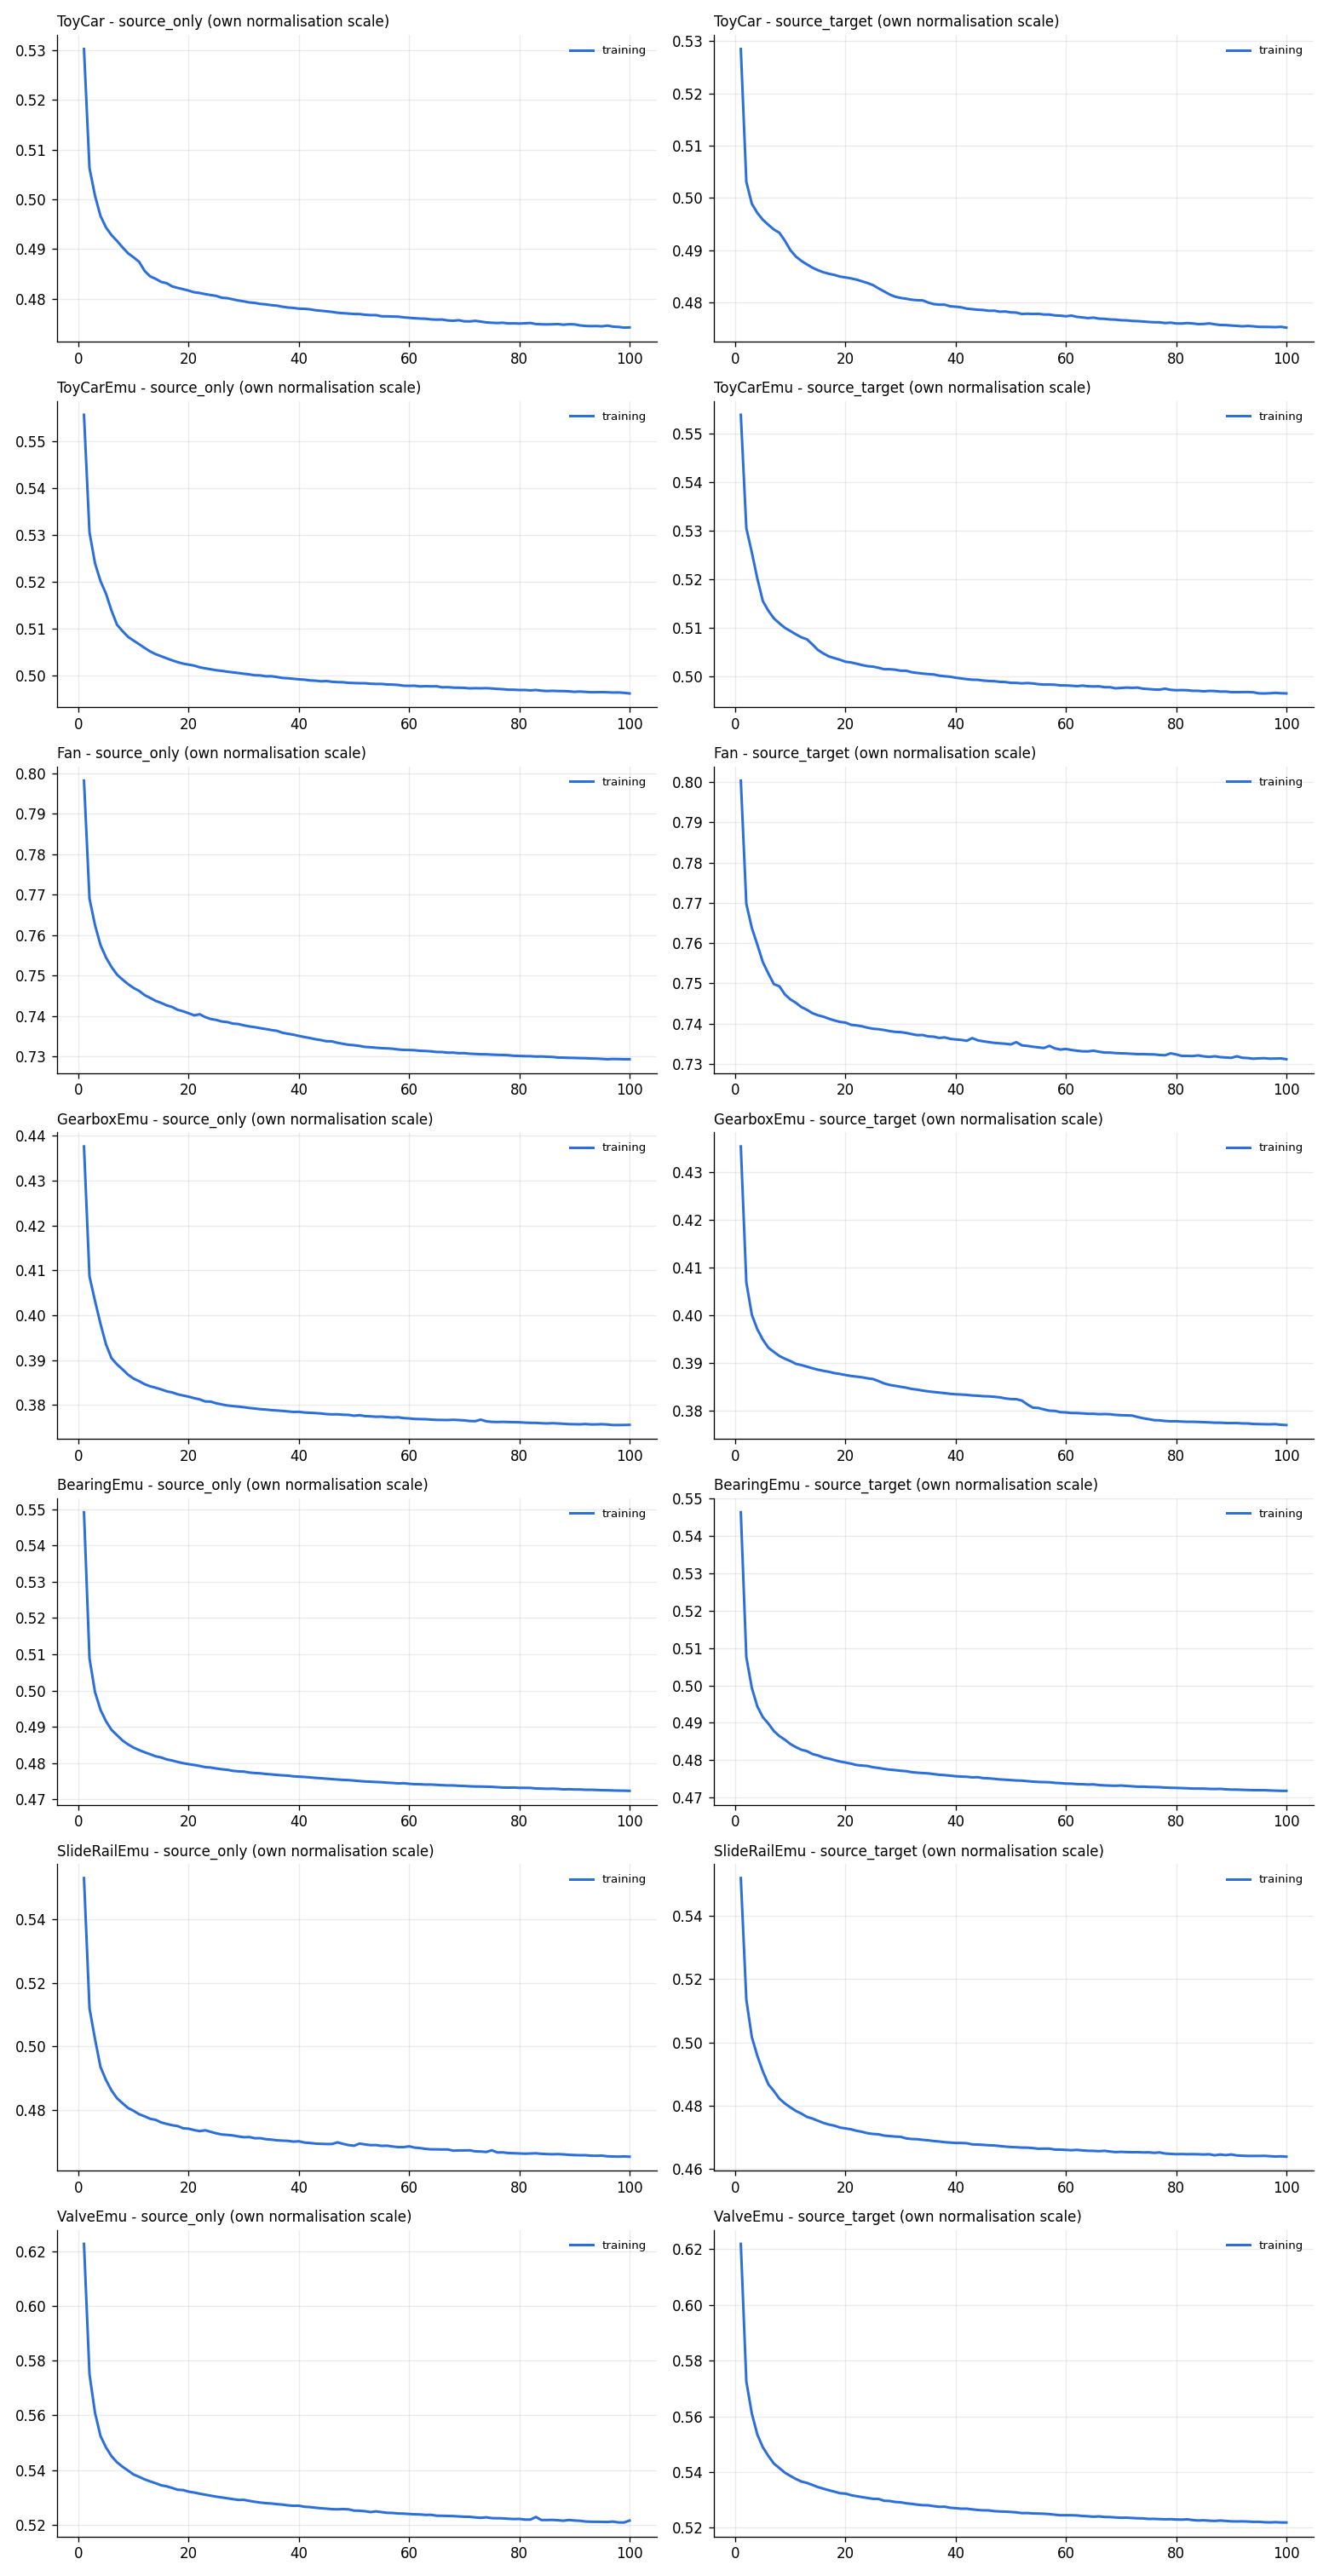
\includegraphics[width=0.96\textwidth,height=0.74\textheight,keepaspectratio]{ALL_MACHINES_loss_curves}
\caption{Training-loss curves of all fourteen models. Rows are machines; the left column is Model~A, the right column Model~B. Each curve is the mean squared error on that model's own standardised features, so values are not comparable across panels.}
\label{fig:losses}
\end{figure}
